\section{Thực nghiệm K-line (Robustness với số lượng cụm $k$)}

\subsection{Mục tiêu của Thực nghiệm}

Thông thường, ta không biết trước dữ liệu nên chia thành bao nhiêu cụm là tốt nhất. Thực nghiệm này đánh giá độ ``lì đòn'' (Robustness) của thuật toán FairDen khi người dùng thay đổi số lượng cụm $k$ từ 2 đến 10.

\subsection{Thiết lập Thực nghiệm}

\textbf{Đối thủ cạnh tranh:}
\begin{itemize}
    \item \textbf{Fairlet (MCF)} và \textbf{Scalable Fair Clustering}: Chỉ hoạt động với thuộc tính nhạy cảm \textbf{nhị phân} (Binary). Nếu thuộc tính có từ 3 giá trị trở lên, các thuật toán này \textbf{không chạy được}.
    \item \textbf{FairDen} và \textbf{FairSC}: Có thể xử lý đa nhóm (Multi-group).
\end{itemize}

\textbf{Cách thực hiện:} Thay đổi $k$ từ 2 đến 10 và đo Balance, DCSI trên tập Adult với:
\begin{itemize}
    \item \textbf{Race} (5 nhóm - adult5): Chỉ có FairDen và FairSC tham gia
    \item \textbf{Gender} (2 nhóm - adult2): Tất cả các thuật toán đều tham gia
\end{itemize}

\subsection{Kết quả của Tác giả}

Hình trong bài báo gốc cho thấy FairDen đạt Balance cao nhất với thuộc tính đa nhóm (Race), và đạt DCSI tốt nhất khi $k$ nhỏ với thuộc tính nhị phân (Gender).

\begin{figure}[H]
\centering
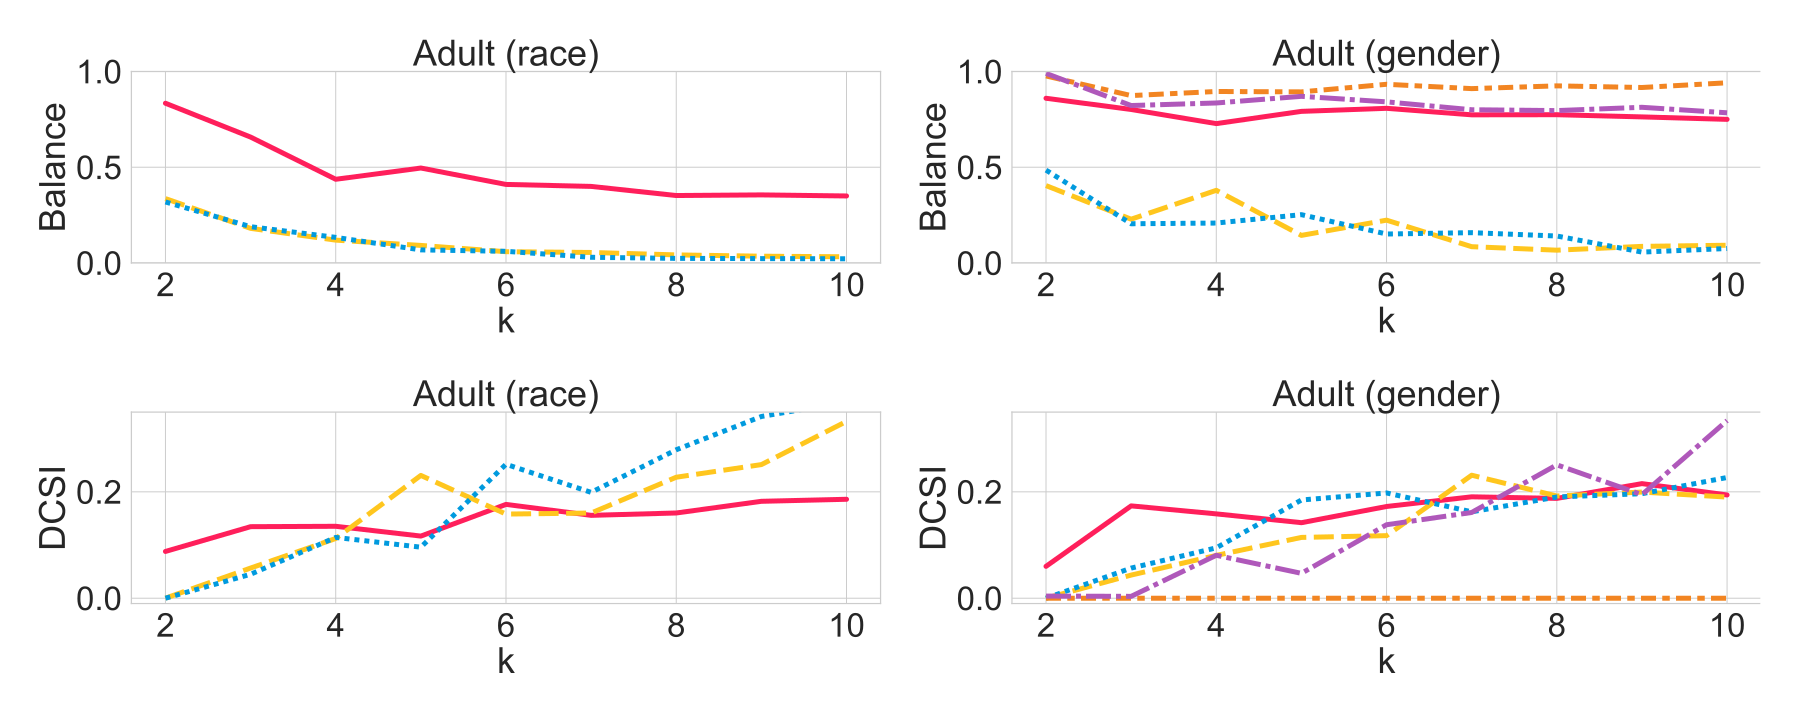
\includegraphics[width=\textwidth]{fig/Lineplot_adult_both.png}
\includegraphics[width=\textwidth]{fig/Legend.png}\\[0.5em]
\caption{Kết quả K-line của tác giả trên tập Adult.}
\label{fig:rw_author}
\end{figure}

\subsection{Kết quả của Nhóm}

\begin{figure}[H]
\centering
\includegraphics[width=\textwidth]{fig/kline_adult_comparison.png}
\caption{Kết quả K-line của nhóm trên tập Adult. Trái: Race (5 nhóm). Phải: Gender (2 nhóm).}
\label{fig:kline_our}
\end{figure}

\begin{figure}[H]
\centering
\includegraphics[width=\textwidth]{fig/kline_compas_comparison.png}
\caption{Kết quả K-line trên tập COMPAS. Trái: Race (4 nhóm). Phải: Sex (2 nhóm).}
\label{fig:kline_compas}
\end{figure}

\subsection{Phân tích Kết quả}

\begin{itemize}
    \item \textbf{Về Balance:}
    \begin{itemize}
        \item FairDen đạt kết quả Balance cao trên các tập dữ liệu thực nghiệm (Adult và COMPAS).
        \item Tuy nhiên, với thuộc tính nhị phân (Gender/Sex), FairDen có Balance thấp hơn so với Fairlet và Scalable như minh họa trong các hình vẽ.
        \item Với thuộc tính đa nhóm (Race), FairDen vượt trội hơn FairSC --- đối thủ duy nhất cũng hỗ trợ đa nhóm.
    \end{itemize}
    
    \item \textbf{Về DCSI:}
    \begin{itemize}
        \item FairDen đạt kết quả DCSI tốt, đặc biệt \textbf{cao vượt trội} trên thực nghiệm COMPAS của nhóm.
        \item Ở các giá trị $k$ lớn, FairDen có DCSI thấp hơn FairSC hoặc Scalable, nhưng vẫn duy trì mức \textbf{ổn định} qua các giá trị $k$ khác nhau.
    \end{itemize}
    
    \item \textbf{Cân bằng và ổn định:}
    \begin{itemize}
        \item Điểm mạnh của FairDen là khả năng \textbf{cân bằng tốt giữa DCSI và Balance}.
        \item Trong khi các thuật toán khác có thể đạt điểm cao hơn ở một chỉ số, FairDen duy trì hiệu suất \textbf{ổn định} trên cả hai chỉ số qua mọi giá trị $k$.
    \end{itemize}
\end{itemize}

\subsection{Kết luận}

\begin{enumerate}
    \item \textbf{Ưu điểm với đa nhóm:} FairDen là lựa chọn số 1 cho các bài toán có thuộc tính nhạy cảm $\geq 3$ nhóm, vì FairSC là đối thủ duy nhất khác có thể xử lý đa nhóm nhưng Balance thấp hơn đáng kể.
    
    \item \textbf{Cân bằng Balance-DCSI:} FairDen không phải lúc nào cũng đạt điểm cao nhất ở từng chỉ số riêng lẻ, nhưng là thuật toán cân bằng và ổn định nhất giữa Balance và DCSI.
    
    \item \textbf{Hiệu quả trên COMPAS:} Kết quả trên tập COMPAS cho thấy FairDen đạt DCSI vượt trội so với các đối thủ, đồng thời duy trì Balance ở mức chấp nhận được.
    
    \item \textbf{Tái hiện thành công:} Xu hướng kết quả của nhóm tương đồng với bài báo gốc, xác nhận tính đúng đắn của thuật toán.
\end{enumerate}
